\resizebox{0.8\columnwidth}{!}{
  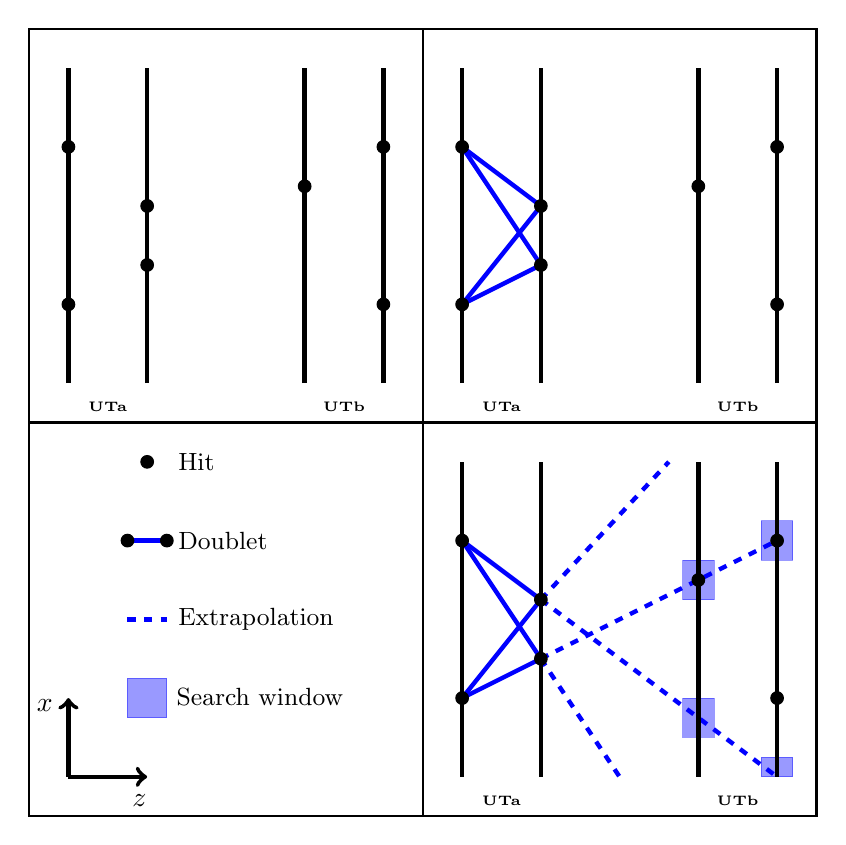
\begin{tikzpicture}
  %\draw[step=1cm,gray,very thin] (0,0) grid (10,10);

  %layout
  \draw[thick] (0,0) rectangle (5,5);
  \draw[thick] (5,0) rectangle (10,5);
  \draw[thick] (0,5) rectangle (5,10);
  \draw[thick] (5,5) rectangle (10,10);

  \draw[thick] (5.0,0.0) -- (5.0,10.0);
  \draw[thick] (0.0,5.0) -- (10.0,5.0);

  %first diagram
  %UT layers
  \draw[ultra thick] (0.5,5.5) -- (0.5,9.5);
  \draw[ultra thick] (1.5,5.5) -- (1.5,9.5);
  \draw[ultra thick] (3.5,5.5) -- (3.5,9.5);
  \draw[ultra thick] (4.5,5.5) -- (4.5,9.5);

  %true hits
  \draw[fill] (0.5,6.5) circle (0.08);
  \draw[fill] (1.5,7.0) circle (0.08);
  \draw[fill] (3.5,8.0) circle (0.08);
  \draw[fill] (4.5,8.5) circle (0.08);

  %fake hits
  \draw[fill] (0.5,8.5) circle (0.08);
  \draw[fill] (1.5,7.75) circle (0.08);
  \draw[fill] (4.5,6.5) circle (0.08);

  %labels
  \node[draw=none] at  (1,5.2){\tiny \bf{UTa}};
  \node[draw=none] at  (4,5.2){\tiny \bf{UTb}};

  %second diagram
  %doublets
  \draw[ultra thick,blue] (5.5,6.5) -- (6.5,7);
  \draw[ultra thick,blue] (5.5,6.5) -- (6.5,7.75);

  \draw[ultra thick,blue] (5.5,8.5) -- (6.5,7);
  \draw[ultra thick,blue] (5.5,8.5) -- (6.5,7.75);

  %UT layers
  \draw[ultra thick] (5.5,5.5) -- (5.5,9.5);
  \draw[ultra thick] (6.5,5.5) -- (6.5,9.5);
  \draw[ultra thick] (8.5,5.5) -- (8.5,9.5);
  \draw[ultra thick] (9.5,5.5) -- (9.5,9.5);

  %true hits
  \draw[fill] (5.5,6.5) circle (0.08);
  \draw[fill] (6.5,7.0) circle (0.08);
  \draw[fill] (8.5,8.0) circle (0.08);
  \draw[fill] (9.5,8.5) circle (0.08);

  %fake hits
  \draw[fill] (5.5,8.5) circle (0.08);
  \draw[fill] (6.5,7.75) circle (0.08);
  \draw[fill] (9.5,6.5) circle (0.08);

  %labels
  \node[draw=none] at  (6,5.2){\tiny \bf{UTa}};
  \node[draw=none] at  (9,5.2){\tiny \bf{UTb}};

  %third diagram
  %doublets
  \draw[ultra thick,blue] (5.5,1.5) -- (6.5,2.0);
  \draw[ultra thick,blue] (5.5,1.5) -- (6.5,2.75);

  \draw[ultra thick,blue] (5.5,3.5) -- (6.5,2.0);
  \draw[ultra thick,blue] (5.5,3.5) -- (6.5,2.75);

  %extrapolations
  %true
  \draw[ultra thick,blue,dashed] (6.5,2.0) -- (9.5,3.5);
  %fake
  \draw[ultra thick,blue,dashed] (6.5,2.0) -- (7.5,0.5);
  \draw[ultra thick,blue,dashed] (6.5,2.75) -- (8.125,4.5);
  \draw[ultra thick,blue,dashed] (6.5,2.75) -- (9.5,0.5);

  %search windows
  %true
  \draw[fill,blue,opacity=0.4] (8.3,2.75) rectangle (8.7,3.25);
  \draw[fill,blue,opacity=0.4] (9.3,3.25) rectangle (9.7,3.75);
  %fake
  \draw[fill,blue,opacity=0.4] (8.3,1.0) rectangle (8.7,1.50);
  \draw[fill,blue,opacity=0.4] (9.3,0.5) rectangle (9.7,0.75);

  %UT layers
  \draw[ultra thick] (5.5,0.5) -- (5.5,4.5);
  \draw[ultra thick] (6.5,0.5) -- (6.5,4.5);
  \draw[ultra thick] (8.5,0.5) -- (8.5,4.5);
  \draw[ultra thick] (9.5,0.5) -- (9.5,4.5);

  %true hits
  \draw[fill] (5.5,1.5) circle (0.08);
  \draw[fill] (6.5,2.0) circle (0.08);
  \draw[fill] (8.5,3.0) circle (0.08);
  \draw[fill] (9.5,3.5) circle (0.08);

  %fake hits
  \draw[fill] (5.5,3.5) circle (0.08);
  \draw[fill] (6.5,2.75) circle (0.08);
  \draw[fill] (9.5,1.5) circle (0.08);

  %labels
  \node[draw=none] at  (6,0.2){\tiny \bf{UTa}};
  \node[draw=none] at  (9,0.2){\tiny \bf{UTb}};

  %legend
  \draw[ultra thick, white] (1.25,4.5) -- (1.75,4.5)  node[anchor=west] {\small \textcolor{black}{Hit}};
  \draw[fill] (1.5,4.5) circle (0.08);

  \draw[ultra thick, blue] (1.25,3.5) -- (1.75,3.5)  node[anchor=west] {\small \textcolor{black}{Doublet}};
  \draw[fill] (1.25,3.5) circle (0.08);
  \draw[fill] (1.75,3.5) circle (0.08);

  \draw[ultra thick, blue,dashed] (1.25,2.5) -- (1.75,2.5) node[anchor=west] {\small \textcolor{black}{Extrapolation}};

  \draw[fill,blue,opacity=0.4,text opacity=1] (1.25,1.25) rectangle (1.75,1.75) node[anchor=north west] {\small \textcolor{black}{Search window}};

  \draw[ultra thick,->] (0.5,0.5) -- (0.5,1.5);
  \draw[ultra thick,->] (0.5,0.5) -- (1.5,0.5);
  \node[draw=none] at  (1.4,0.2){$z$};
  \node[draw=none] at  (0.2,1.4){$x$};

  \end{tikzpicture}
}
   